\documentclass[a4paper,12pt]{article}

% Import the deliverable package from common directory
\usepackage{../common/deliverable}

% Tell LaTeX where to find graphics files
\graphicspath{{../common/logos/}{./figures/}{../}}

\usepackage{xspace}
\usepackage{lipsum}

% --- Packages ---
\usepackage[utf8x]{inputenc}    % Input encoding (allows international characters)
\usepackage{listings}
\usepackage{graphicx}          % Include images

% Set the deliverable number (without the D prefix, it's added automatically)
\setdeliverableNumber{3.4}

% Begin document
\begin{document}

% Create the title page with the title as argument
\maketitlepage{Co-Design and Energy Efficiency Report - II}

\newpage

% Main Table using the new environment and command
\begin{deliverableTable}
    \tableEntry{Deliverable title}{Co-Design and Energy Efficiency Report - II}
    \tableEntry{Deliverable number}{D3.4}
    \tableEntry{Deliverable version}{v1}
    \tableEntry{Date of delivery}{July 31, 2026}
    \tableEntry{Actual date of delivery}{July 31, 2026}
    \tableEntry{Nature of deliverable}{[Report]}
    \tableEntry{Dissemination level}{[Public]}
    \tableEntry{Work Package}{WP2}
    \tableEntry{Partner responsible}{LRZ}
\end{deliverableTable}

% Abstract and Keywords Section
\begin{deliverableTable}
    \tableEntry{Abstract}{This report focuses on development and porting of finite element kernels to GPU architectures and analysis of energy efficiency.}
    \tableEntry{Keywords}{codesign; performance; energy}
\end{deliverableTable}

\newpage

\begin{documentControl}
    \addVersion{0.1}{29/06/2026}{Ivan Pribec}{Initial draft}
    \addVersion{0.2}{[Date]}{[Author name]}{[Description of changes]}
    \addVersion{0.3}{[Date]}{[Author name]}{[Description of changes]}
    \addVersion{1.0}{[Date]}{[Author name]}{Final version}
\end{documentControl}

\subsection*{{Approval Details}}
Approved by: [Name] \\
Approval Date: [Date]

\subsection*{{Distribution List}}
\begin{itemize}
    \item [] - Project Coordinators (PCs)
    \item [] - Work Package Leaders (WPLs)
    \item [] - Steering Committee (SC)
    \item [] - European Commission (EC)
\end{itemize}

\vspace*{2cm}

\disclaimer

\newpage

\tableofcontents % Automatically generated and hyperlinked Table of Contents

\newpage

\section{{Introduction}}

\lipsum[1-2]

\subsection{{Purpose of the Document}}
\lipsum[3]

\subsection{{Structure of the Document}}
\begin{itemize}
    \item Section \ref{sec:section2}: [Section Title]
    \item Section \ref{sec:section3}: [Section Title]
    \item Section \ref{sec:section4}: [Section Title]
    \item Section \ref{sec:section5}: [Section Title]
    \item Section \ref{sec:section6}: [Section Title]
\end{itemize}

\newpage

\section{{[Section Title]}}
\label{sec:section2}

\lipsum[4-5]

\subsection{{[Subsection Title]}}
\lipsum[6]

\subsection{{[Subsection Title]}}
\lipsum[7]

\newpage


\section{{Performance Evaluations of High Order Finite Element Kernels on Modern Accelerators}}
\label{sec:section3}

We detail the implementation techniques and performance measurements of high-order matrix-free finite element methods on modern graphics processing units (GPUs).
The matrix-free framework and its initial implementations are described in Deliverable 1.3 (\url{https://github.com/dealii-X/deliverables/blob/main/D1.3/D1.3_dealii_report.pdf}).
To evaluate these problems, we adopt the bake-off benchmarks \cite{bakeoff} as our baseline problems. In this report, we also implement a new technique to improve operator performance for low-order elements.
Previous high-order matrix-free GPU implementations were based on assigning a single element per thread block \cite{tens_prod}. This approach causes low-order elements to underutilize
the streaming multiprocessors (SMs) because NVIDIA only allows each SM to schedule 32 thread blocks \cite{nvidia_hopper_tuning}. Consequently, low-order elements reach this limit,
leaving registers and shared memory underutilized within each SM. On AMD GPUs, the single element per thread block approach leaves the 64-thread wavefront underutilized for low-order elements, consequently causing poor performance.
Based on a batch processing approach, our technique assigns multiple elements to each thread block to overcome these limitations. For example, a polynomial order of 1 in the Laplace operator evaluation (Bake-Off Kernel 3 in the CEED benchmarks) can fit 11 elements per thread block.
A performance comparison between the single-element-per-thread-block and the batched processing approaches is given in Figure~\ref{fig:BK3_1_10}. The new technique achieves a 2$\times$ speedup for polynomial order 1 on the NVIDIA GH200 Superchip at the JUPITER supercomputer located at the Jülich Research Centre.
New batched implementations are available at \url{https://github.com/dealii-X/benchmarks/tree/main/CEED\_BK}.

\subsection{Experimental Setup}
Performance analysis and benchmarks were conducted on the NVIDIA Grace Hopper Superchip (GH200) on the JUPITER supercomputer and on the AMD MI250X GPU on the LUMI supercomputer. The Kokkos performance portability layer
v5.1 \cite{Kokkos} was used to target traditional compute cores. For tensor core implementations, CUDA PTX mma instructions v9.3 \cite{nvidia_mma} were employed.

\subsection{Operator Performance and Optimization Analysis}
\begin{figure}[htbp]
    \centering
    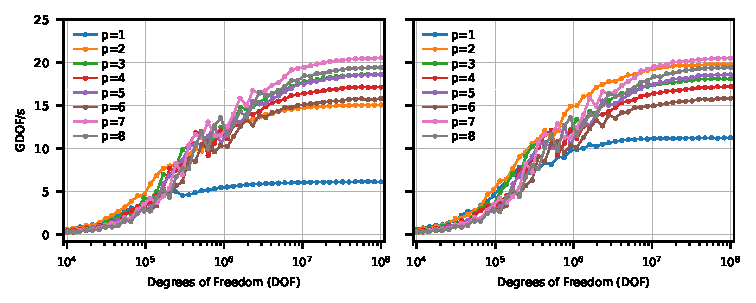
\includegraphics[width=0.9\textwidth]{figures/GH200_fp64_BK3_1KB_10KB}
    \caption{Performance comparison of the Laplace operator (BK3) in FP64 on the NVIDIA GH200. Single-element-per-thread-block approach (Left); proposed multiple-elements-per-thread-block approach (right).}
    \label{fig:BK3_1_10}
\end{figure}

To see the occupancy impact of our proposed approach, we investigate the performance of 12.5 million linear elements ($p=1$) in double precision using the NVIDIA Nsight Compute profiler.
Figure~\ref{fig:occ_1kb} shows a screenshot of the occupancy calculator for the single element per thread block kernel. Each box represents a thread block, where light blue boxes represent
allocated blocks and dark blue boxes represent unallocated blocks. We can clearly see that 18.8\% of registers and 31\% of shared memory are left unused due to the 32-thread-block-per-SM limit.
On the other hand, Figure~\ref{fig:occ_10kb} shows 10 allocated blocks. In this case, higher register usage becomes the occupancy limiter, resulting in improved performance.

\begin{figure}[htbp]
    \centering
    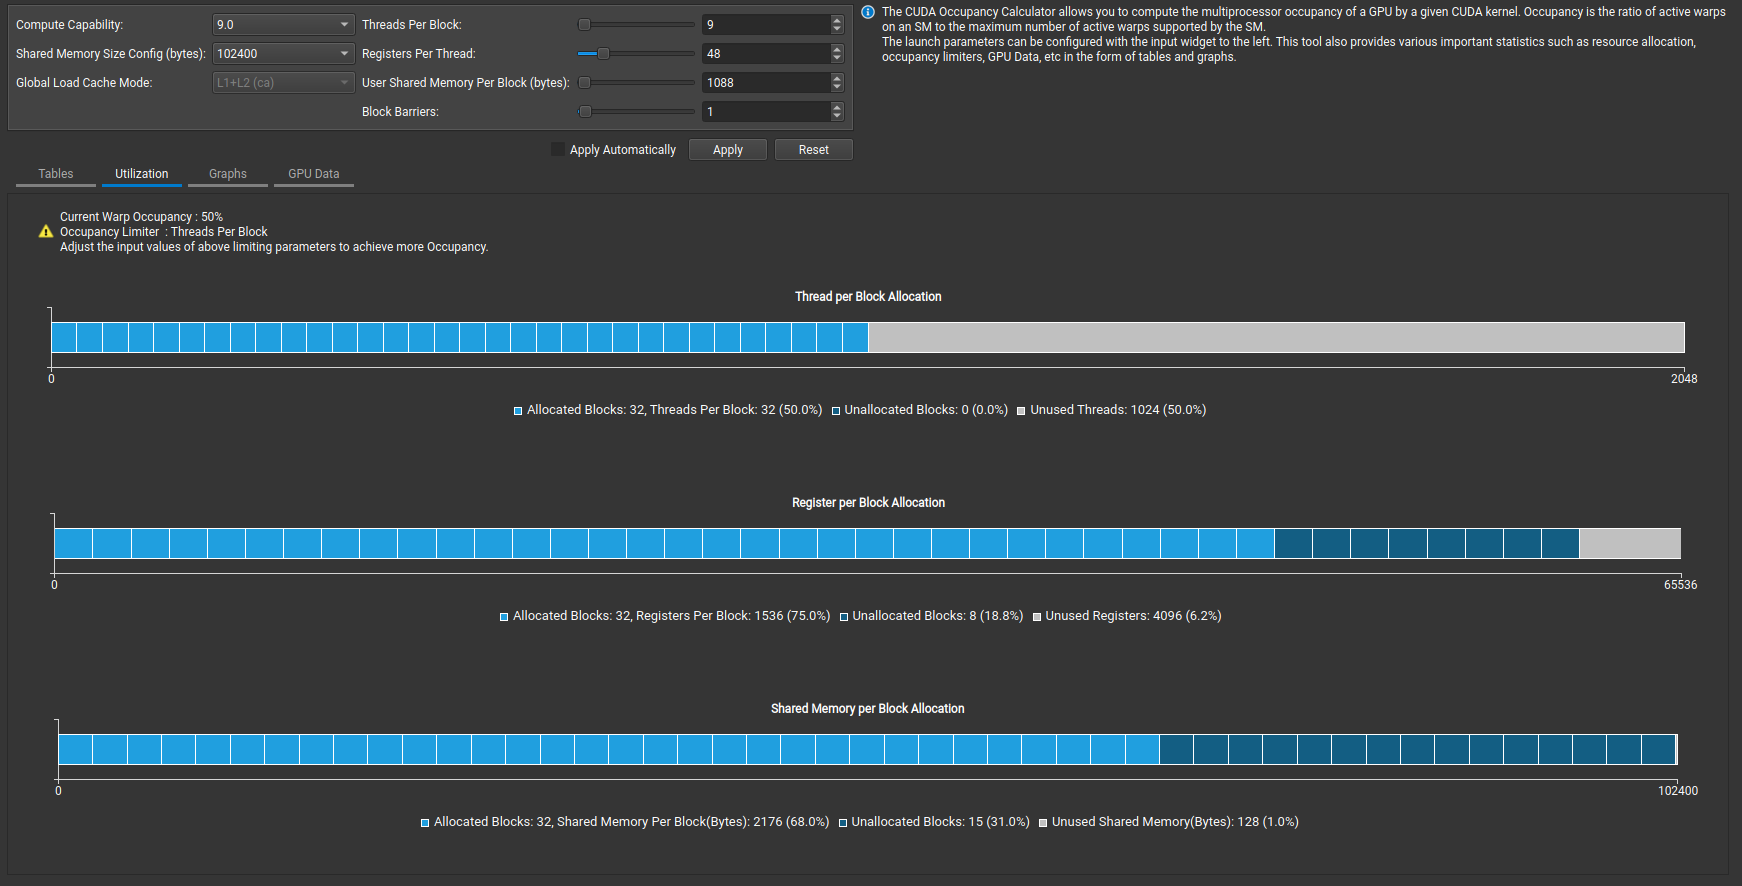
\includegraphics[width=0.9\textwidth]{figures/Occ_1KB}
    \caption{Occupancy calculator screenshot from NVIDIA Nsight Compute for the single element per thread block technique on laplace kernel, evaluated using 12.5 million linear elements in double precision.}
    \label{fig:occ_1kb}
\end{figure}

\begin{figure}[htbp]
    \centering
    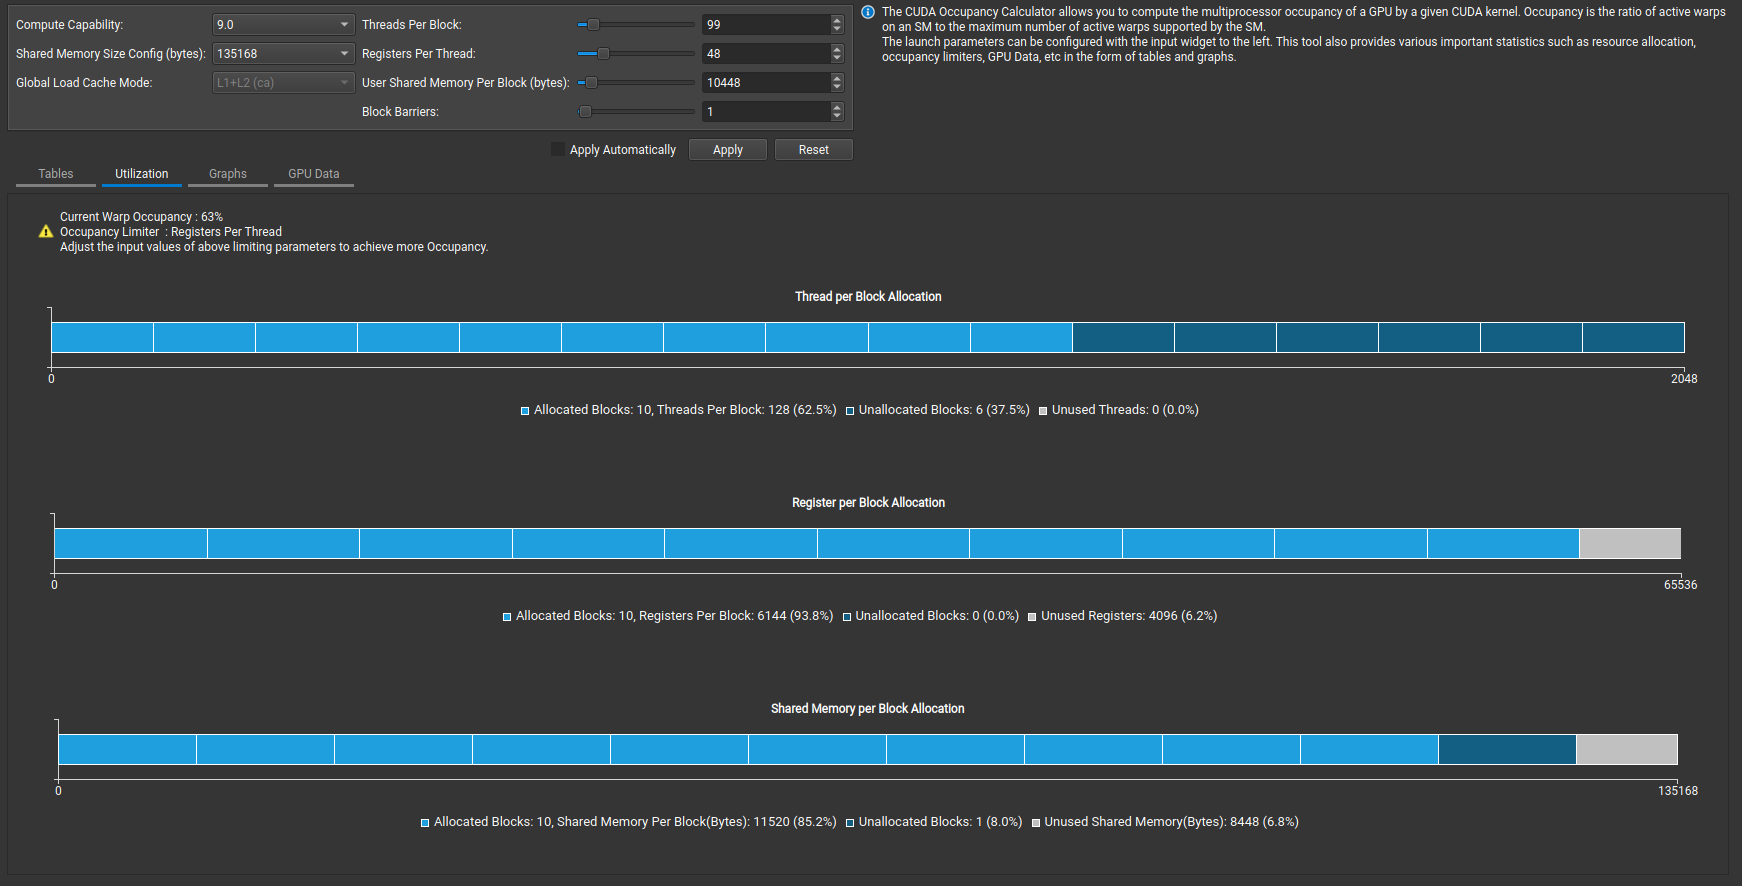
\includegraphics[width=0.9\textwidth]{figures/Occ_10KB}
    \caption{Occupancy calculator screenshot from NVIDIA Nsight Compute for the batched processing technique on laplace kernel, evaluated using 12.5 million linear elements in double precision.}
    \label{fig:occ_10kb}
\end{figure}

To further analyze performance, we also leveraged NVIDIA Nsight Compute’s roofline model to effectively compare a kernel's achieved performance with the hardware bandwidth and FLOP/s limits.
Figure~\ref{fig:roof_1kb} shows the hierarchical roofline model for the single element per thread block technique, evaluated with the same 12.5 million linear element Laplace kernel.
The plot includes the L1, L2 and global memory bandwidth boundaries. On this target GH200 GPU, the streaming global memory bandwidth is 3.6 TB/s, whereas its theoretical FP64 peak performance is 33 TFLOPS.
Due to the low arithmetic intensity of low-order elements in matrix-free methods, polynomial order 1 has an global memory arithmetic intensity of only 1.3~FLOP/B, achieving a performance of 1.4 TFLOPS.
This achieves only 27\% of the theoretical roofline limit (5.2 TFLOPS) at that arithmetic intensity. In contrast, the batched processing approach achieves 2.5~TFLOPS at the same arithmetic intensity, reaching 48\%
of the theoretical throughput limit.

\begin{figure}[htbp]
    \centering
    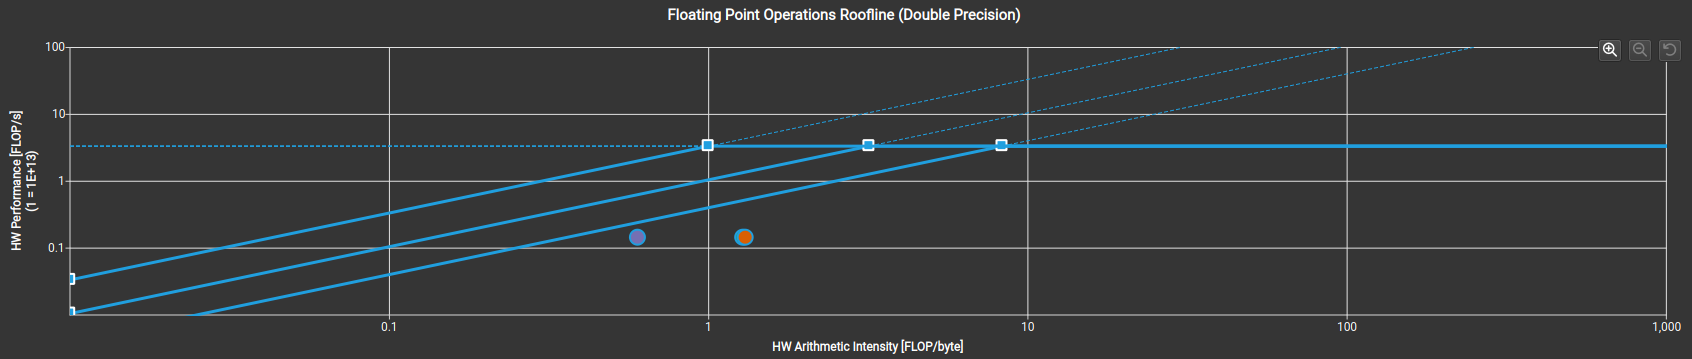
\includegraphics[width=0.9\textwidth]{figures/roof_1KB}
    \caption{Roofline model from NVIDIA Nsight Compute for the single element per thread block laplace kernel, evaluated using 12.5 million linear elements in double precision.
    The kernel achieves an arithmetic intensity of 1.3 FLOP/B in global memory and a performance of 1.4 TFLOPS (green solid circle), corresponding to 27\% of the theoretical roofline limit (5.2 TFLOPS) at this
    arithmetic intensity.}
    \label{fig:roof_1kb}
\end{figure}

\begin{figure}[htbp]
    \centering
    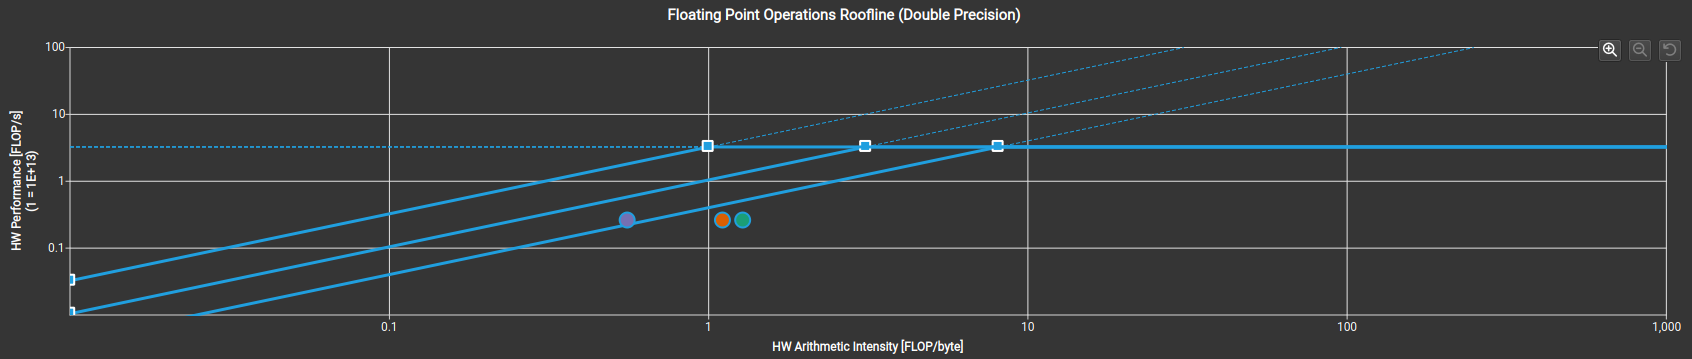
\includegraphics[width=0.9\textwidth]{figures/roof_10KB}
    \caption{Roofline model from NVIDIA Nsight Compute for the batch processing laplace kernel, evaluated using 12.5 million linear elements in double precision.
    The kernel achieves an arithmetic intensity of 1.3 FLOP/B in global memory and a performance of 2.5 TFLOPS (green solid circle), corresponding to 48\% of the theoretical roofline limit (5.2 TFLOPS) at this
    arithmetic intensity.}
    \label{fig:roof_10kb}
\end{figure}

\subsection{Laplace Solver Performance (CEED BP3)}
We extend our operator evaluation to a complete linear solver by embedding the Laplace operator within a Conjugate Gradient (CG) method, corresponding to the CEED Bake-Off Problem 3 (BP3) benchmark.
The solver, implemented within the deal.II finite element library framework is evaluated on both single and multi-GPU configurations of the NVIDIA GH200 Superchip, utilizing MPI with peer-to-peer (P2P) communication enabled. Figure~\ref{fig:BK_BP} illustrates the initial performance results,
highlighting that the performance difference between operator evaluations (BK) and full linear solvers (BP)
is primarily driven by gather-scatter overheads and inter-GPU communication. Additionally, the results confirm the computational efficiency of high-order elements which directly leverages the tensor-product formulation of the shape functions to increase arithmetic intensity.
The source code can be found at \url{https://github.com/dealii-X/benchmarks/tree/main/CEED_bp}.

\begin{figure}[htbp]
    \centering
    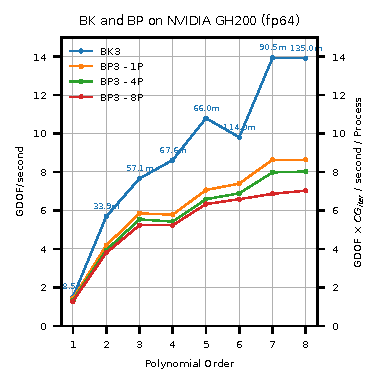
\includegraphics[width=0.5\textwidth]{figures/GH200_BK_BP}
    \caption{
        Performance results for the Laplace Operator (CEED BK3) \& Problem (CEED BP3) are evaluated across various polynomial orders and problem sizes on the GH200 GPU. Both Bake-Off Kernel performance (GDOF/s)
        and Bake-Off Problem performance ($\text{GDOF} \times \text{CG}_{\text{iter}} / (\text{second} \times \text{process})$) are measured using the global degrees of freedom (the T-vector in CEED).
    }
    \label{fig:BK_BP}
\end{figure}

\subsection{Raviart-Thomas Elements and Kernel Performance}
$H^1$-conforming elements (as used in the CEED Bake-Off kernels) enforce continuity of all vector components across elements, whereas the Navier-Stokes equations,
in mixed formulations often require continuity of the normal component of the flux across element boundaries which is a property of $H(\mathrm{div})$-conforming spaces.
Elements designed for this purpose are known as Raviart-Thomas finite elements. We developed the vector Mass, mixed divergence and mixed gradient operators the core operations
in Raviart-Thomas kernel design and implemented them in our benchmarks. These benchmarks are available at \url{https://github.com/dealii-X/benchmarks/tree/main/rt\_kernels}.

Figure \ref{fig:GH200_vector_Mass} shows the performance of the vector Mass operator on the NVIDIA GH200 in both FP32 and FP64 precisions. Batch processing enabled all polynomial orders to achieve similar throughput (GDOF/s). Similar trends are observed for the AMD MI250X
GPU from the LUMI supercomputer, which performs well given its $1.3\text{ TB/s}$ STREAM bandwidth. Only polynomial order 8 performs significantly worse than the other orders, as shown in Figure \ref{fig:MI250x_vector_Mass}.
This drop in performance is likely due to register file capacity constraints in this slightly older AMD architecture.

\begin{figure}[htbp]
    \centering
    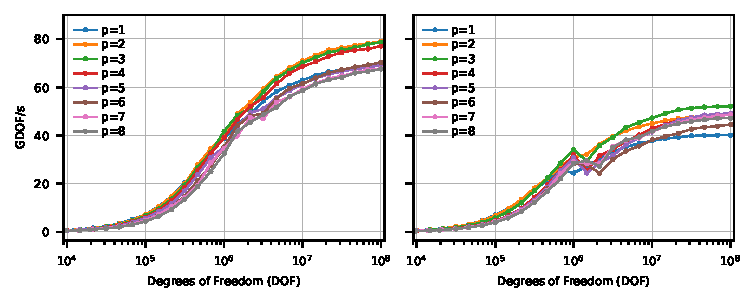
\includegraphics[width=0.9\textwidth]{figures/GH200_Mass_32_64}
    \caption{Performance comparison of the vector Mass operator using FP32 (left) and FP64 (right) precisions on the NVIDIA GH200 Superchip.}
    \label{fig:GH200_vector_Mass}
\end{figure}

\begin{figure}[htbp]
    \centering
    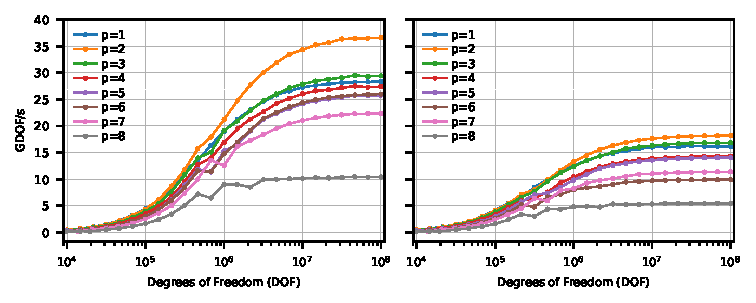
\includegraphics[width=0.9\textwidth]{figures/MI250x_Mass_32_64}
    \caption{Performance comparison of the vector Mass operator using FP32 (left) and FP64 (right) precisions on the single AMD MI250x GPU tile.}
    \label{fig:MI250x_vector_Mass}
\end{figure}


We also introduce a new technique to target NVIDIA tensor cores \cite{nvidia_mma}
which are designed to perform fast matrix-matrix multiplication in different precisions. Initial implementations for FP64 and non-IEEE-compliant TensorFloat-32 (TF32) are available
in the same rt\_kernels benchmarks repository.


\section{{[Section Title]}}
\label{sec:section5}

\lipsum[14-15]

\subsection{{[Subsection Title]}}
\lipsum[16]

\subsection{{[Subsection Title]}}
\begin{itemize}[left=1em, itemsep=0pt, topsep=0pt] 
    \item \textbf{[Item Title]}: \lipsum[17][1-2]
    \item \textbf{[Item Title]}: \lipsum[17][3-4]
    \item \textbf{[Item Title]}: \lipsum[17][5-6]
\end{itemize}

\newpage

\section{{[Section Title]}}
\label{sec:section6}

\lipsum[18-19]

\begin{center}
\resizebox{\textwidth}{!}{
\begin{tabular}{|l|l|l|}
\hline
\textbf{Column 1} & \textbf{Column 2} & \textbf{Column 3} \\
\hline
Item 1 & Description & Value \\
\hline
Item 2 & Description & Value \\
\hline
Item 3 & Description & Value \\
\hline
\end{tabular}}
\label{tab:example_table2}
\end{center}

\newpage 

\section{{Conclusion}} \label{sec:conclusion}

\lipsum[20]

\label{MyLastPage}

%\clearpage
%\bibliographystyle{plainurl}
%\bibliography{references}

\end{document}
